\documentclass[9pt,twocolumn,twoside,]{pnas-new}

%% Some pieces required from the pandoc template
\providecommand{\tightlist}{%
  \setlength{\itemsep}{0pt}\setlength{\parskip}{0pt}}

% Use the lineno option to display guide line numbers if required.
% Note that the use of elements such as single-column equations
% may affect the guide line number alignment.


\usepackage[T1]{fontenc}
\usepackage[utf8]{inputenc}

% Pandoc citation processing


\templatetype{pnasresearcharticle}  % Choose template

\title{Template para preparar tu trabajo final para la presentación}

\author[a,1,2]{Alice Anonymous}
\author[a,b]{Bob Security}

  \affil[a]{Some Institute of Technology, Department, Street, City, State, Zip}
  \affil[b]{Another University Department, Street, City, State, Zip}


% Please give the surname of the lead author for the running footer
\leadauthor{Anonymous}

% Please add here a significance statement to explain the relevance of your work
\significancestatement{Authors must submit a 120-word maximum statement about the significance
of their research paper written at a level understandable to an
undergraduate educated scientist outside their field of speciality. The
primary goal of the Significance Statement is to explain the relevance
of the work in broad context to a broad readership. The Significance
Statement appears in the paper itself and is required for all research
papers.}


\authorcontributions{Please provide details of author contributions here.}



\correspondingauthor{\textsuperscript{2} To whom correspondence should be addressed. E-mail:
\href{mailto:bob@email.com}{\nolinkurl{bob@email.com}}}

% Keywords are not mandatory, but authors are strongly encouraged to provide them. If provided, please include two to five keywords, separated by the pipe symbol, e.g:
 \keywords{  one |  two |  optional |  optional |  optional  } 

\begin{abstract}
Please provide an abstract of no more than 250 words in a single
paragraph. Abstracts should explain to the general reader the major
contributions of the article. References in the abstract must be cited
in full within the abstract itself and cited in the text.
\end{abstract}

\dates{This manuscript was compiled on \today}
\doi{\url{www.pnas.org/cgi/doi/10.1073/pnas.XXXXXXXXXX}}

\begin{document}

% Optional adjustment to line up main text (after abstract) of first page with line numbers, when using both lineno and twocolumn options.
% You should only change this length when you've finalised the article contents.
\verticaladjustment{-2pt}

\maketitle
\thispagestyle{firststyle}
\ifthenelse{\boolean{shortarticle}}{\ifthenelse{\boolean{singlecolumn}}{\abscontentformatted}{\abscontent}}{}

% If your first paragraph (i.e. with the \dropcap) contains a list environment (quote, quotation, theorem, definition, enumerate, itemize...), the line after the list may have some extra indentation. If this is the case, add \parshape=0 to the end of the list environment.

\acknow{Please include your acknowledgments here, set in a single paragraph.
Please do not include any acknowledgments in the Supporting Information,
or anywhere else in the manuscript.}

This template is provided to help you write your work in the correct
journal format. Instructions for use are provided below.

Note: please start your introduction without including the word
``Introduction'' as a section heading (except for math articles in the
Physical Sciences section); this heading is implied in the first
paragraphs.

\hypertarget{guide-to-using-this-template}{%
\section*{Guide to using this
template}\label{guide-to-using-this-template}}
\addcontentsline{toc}{section}{Guide to using this template}

Please note that whilst this template provides a preview of the typeset
manuscript for submission, to help in this preparation.

\hypertarget{author-affiliations}{%
\subsection*{Author Affiliations}\label{author-affiliations}}
\addcontentsline{toc}{subsection}{Author Affiliations}

Include group, generation and year

\hypertarget{format}{%
\subsection*{Format}\label{format}}
\addcontentsline{toc}{subsection}{Format}

Many authors find it useful to organize their manuscripts with the
following order of sections; Title, Author Affiliation, Keywords,
Abstract, Significance Statement, Results, Discussion, Materials and
methods, Acknowledgments, and References. Other orders and headings are
permitted.

\hypertarget{manuscript-length}{%
\subsection*{Manuscript Length}\label{manuscript-length}}
\addcontentsline{toc}{subsection}{Manuscript Length}

This format uses a two-column format averaging 67 characters, including
spaces, per line.

\hypertarget{references}{%
\subsection*{References}\label{references}}
\addcontentsline{toc}{subsection}{References}

References should be cited in numerical order as they appear in text;
this will be done automatically via bibtex, e.g.~(1) and (2, 3). All
references, including for the SI, should be included in the main
manuscript file. References appearing in both sections should not be
duplicated. SI references included in tables should be included with the
main reference section.

\begin{figure}
\centering
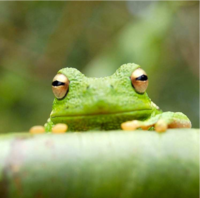
\includegraphics{frog.png}
\caption{Placeholder image of a frog with a long example caption to show
justification setting.{}}
\end{figure}

\hypertarget{sec:figures}{%
\subsection*{Digital Figures}\label{sec:figures}}
\addcontentsline{toc}{subsection}{Digital Figures}

Figures and Tables should be labelled and referenced in the standard way
using the \texttt{\textbackslash{}label\{\}} and
\texttt{\textbackslash{}ref\{\}} commands.

Figure \[fig:frog\] shows an example of how to insert a column-wide
figure. To insert a figure wider than one column, please use the
\texttt{\textbackslash{}begin\{figure*\}...\textbackslash{}end\{figure*\}}
environment. Figures wider than one column should be sized to 11.4 cm or
17.8 cm wide.

\hypertarget{single-column-equations}{%
\subsection*{Single column equations}\label{single-column-equations}}
\addcontentsline{toc}{subsection}{Single column equations}

Authors may use 1- or 2-column equations in their article, according to
their preference.

To allow an equation to span both columns, options are to use the
\texttt{\textbackslash{}begin\{figure*\}...\textbackslash{}end\{figure*\}}
environment mentioned above for figures, or to use the
\texttt{\textbackslash{}begin\{widetext\}...\textbackslash{}end\{widetext\}}
environment as shown in equation \[eqn:example\] below.

Please note that this option may run into problems with floats and
footnotes, as mentioned in the \href{http://texdoc.net/pkg/cuted}{cuted
package documentation}. In the case of problems with footnotes, it may
be possible to correct the situation using commands
\texttt{\textbackslash{}footnotemark} and
\texttt{\textbackslash{}footnotetext}.

\[\begin{aligned}
(x+y)^3&=(x+y)(x+y)^2\\
       &=(x+y)(x^2+2xy+y^2) \label{eqn:example} \\
       &=x^3+3x^2y+3xy^3+x^3. 
\end{aligned}\]

\hypertarget{appendices}{%
\subsubsection*{Appendices}\label{appendices}}
\addcontentsline{toc}{subsubsection}{Appendices}

It is possible to add supplementary information to clarify the content,
But they must be short and summarized.

\hypertarget{set_bibio}{%
\subsubsection*{Setting Bibliography}\label{set_bibio}}
\addcontentsline{toc}{subsubsection}{Setting Bibliography}

The bibliography must be added into an bib file in order to allow latex
to generate bibliography.

\showmatmethods
\showacknow
\pnasbreak

\hypertarget{refs}{}
\leavevmode\hypertarget{ref-belkin2002using}{}%
1. Belkin M, Niyogi P (2002) Using manifold stucture for partially
labeled classification. \emph{Advances in Neural Information Processing
Systems}, pp 929--936.

\leavevmode\hypertarget{ref-berard1994embedding}{}%
2. Bérard P, Besson G, Gallot S (1994) Embedding riemannian manifolds by
their heat kernel. \emph{Geometric \& Functional Analysis GAFA}
4(4):373--398.

\leavevmode\hypertarget{ref-coifman2005geometric}{}%
3. Coifman RR, et al. (2005) Geometric diffusions as a tool for harmonic
analysis and structure definition of data: Diffusion maps.
\emph{Proceedings of the National Academy of Sciences of the United
States of America} 102(21):7426--7431.



% Bibliography
% \bibliography{pnas-sample}

\end{document}

